\documentclass{article}

\usepackage{../../common/labconfig}
\usepackage{../../common/labstyle}

\lhead{UART Lab}

\begin{document}

\section{Introduction}

In this lab, you will learn the basis of interfacing with the UART controller
of the ATMega328P. You will first implement a simple "LED blink" program in
Part A. In Part B, you will implement a "hello world" program. Finally in Part
C you will combine the two into an interactive console program to control the
LED.

This project is split into three parts, which are graded separately. This is
intended to ensure that you are making progress on the project throughout the
allocated time, and to help get you feedback as quickly as possible.
Additionally, you will write a brief reflection on this assignment by
responding to several free-response questions.

\textbf{You will turn in one single file at the end of part C, and another at
part D, which will be generated by running the command \texttt{make pack}. This
file will automatically include your code and your reflection responses.
Incorrectly packed submissions will not be graded.}

Note that \texttt{make pack} requires you to have modified the
\texttt{reflection.txt} file, but the reflection will not be graded until after
Part D is turned in. If you have not started it by the time you submit Part C,
you can simply add one line of text indicating this.

\begin{figure}[H]

	\centering

	\begin{tabular}{r|l}

		Part & Due Date \\ \hline\hline
		Part A & TBD \\ \hline
		Part B & TBD \\ \hline
		Part C & TBD \\ \hline
		Part D & TBD \\ \hline
		Reflection & TBD \\ \hline

	\end{tabular}

	\caption{Table of due dates for each part.}

\end{figure}

\tableofcontents

\section{Parts List}

\begin{multicols}{2}

\begin{itemize}

\item one Arduino UNO\footnote{Or compatible development board with an ATMega328P.}

\item one LED

\item several male-male jumper wires

\item one USB cable

\item one breadboard

\item one 330$\Omega$ resistor (orange, orange, brown, gold)\footnote{Larger
	resistor may be substituted if needed.}

\item AVRIce Programmer and cables

\end{itemize}

\end{multicols}

\begin{figure}[H]
	\centering

	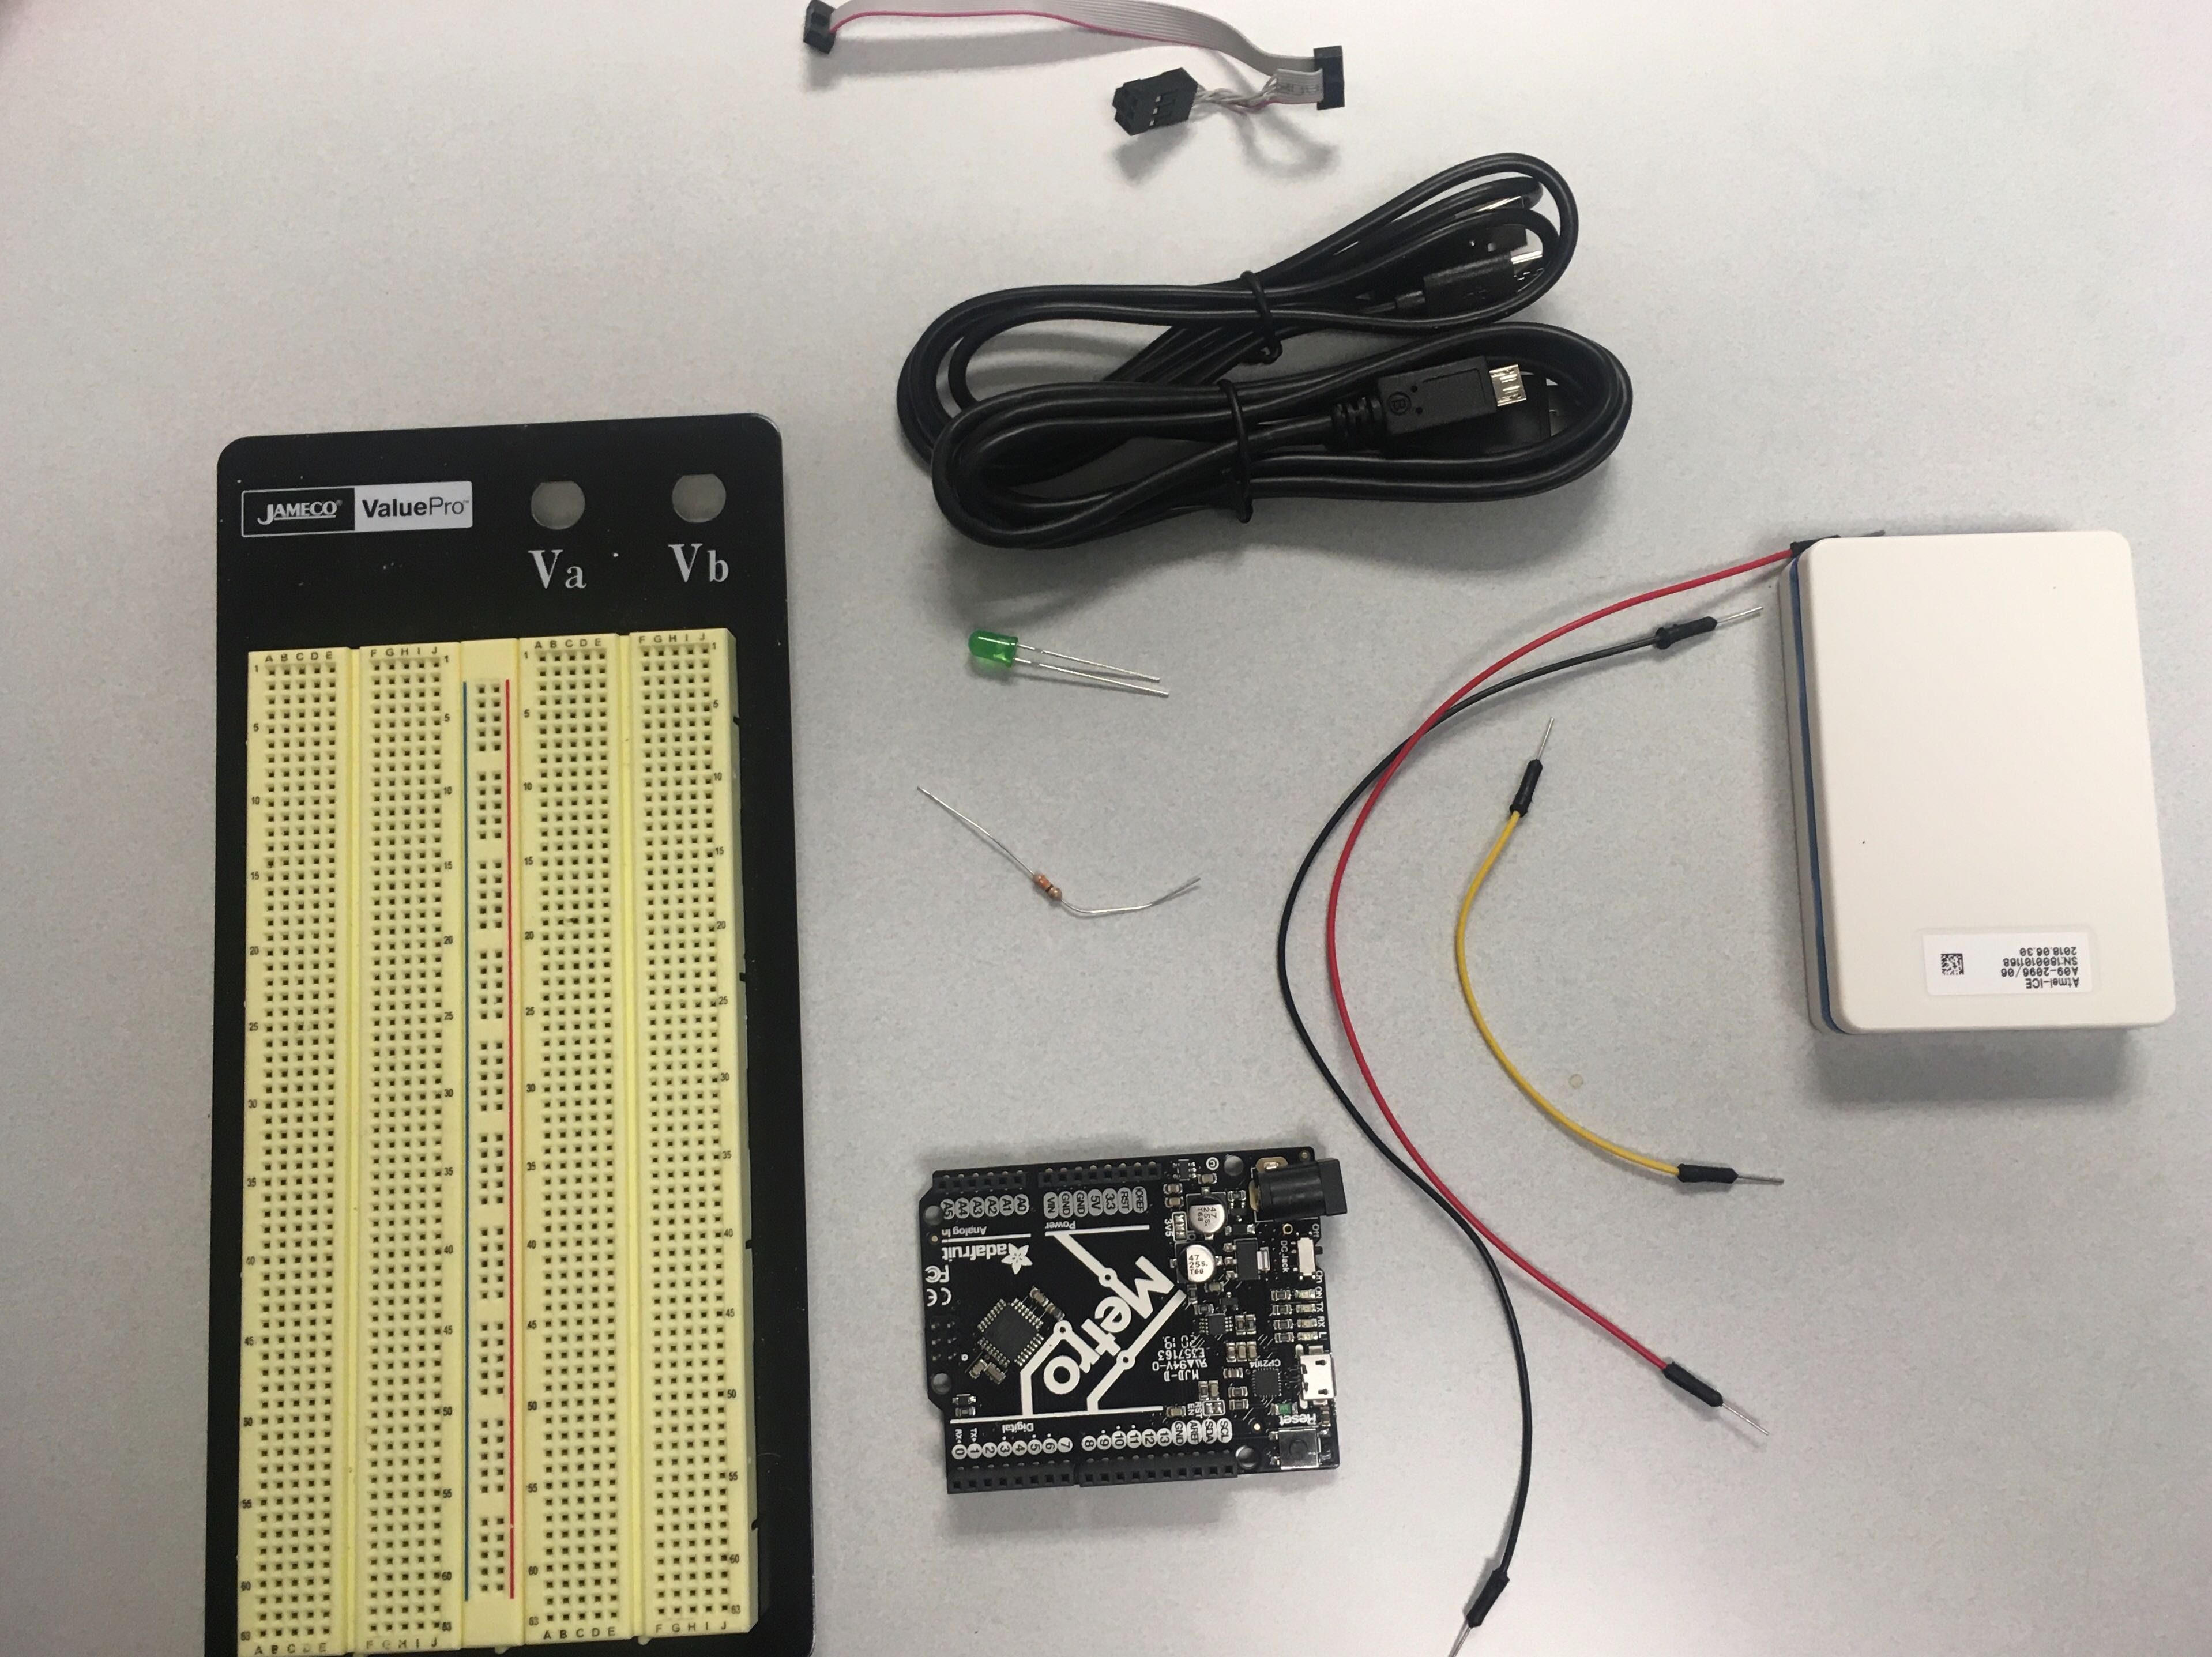
\includegraphics[max width = 0.7\textwidth]{parts.jpg}

	\caption{Photo showing parts for this project.}

\end{figure}

\textbf{NOTE:} this document is written assuming you are using PC0 to drive the
LED. You can use a different pin, but you will also have to account for this
when writing your code.

\section{Part A: LED Blink}

\subsection{Wiring}

Connect the LED to PC0 (marked as A0 on the Arduino). The anode (long leg)
should connect to PC0. Connect the short leg of the LED (the cathode) to ground
via the resistor.

\textbf{TIP:} If you can't tell which leg is longer (for example, if you have
trimmed the legs on the LED), the side of the LED with the shorter leg
(cathode) is also slightly flattened near the base of the LED.

\begin{figure}[H]
	\centering

	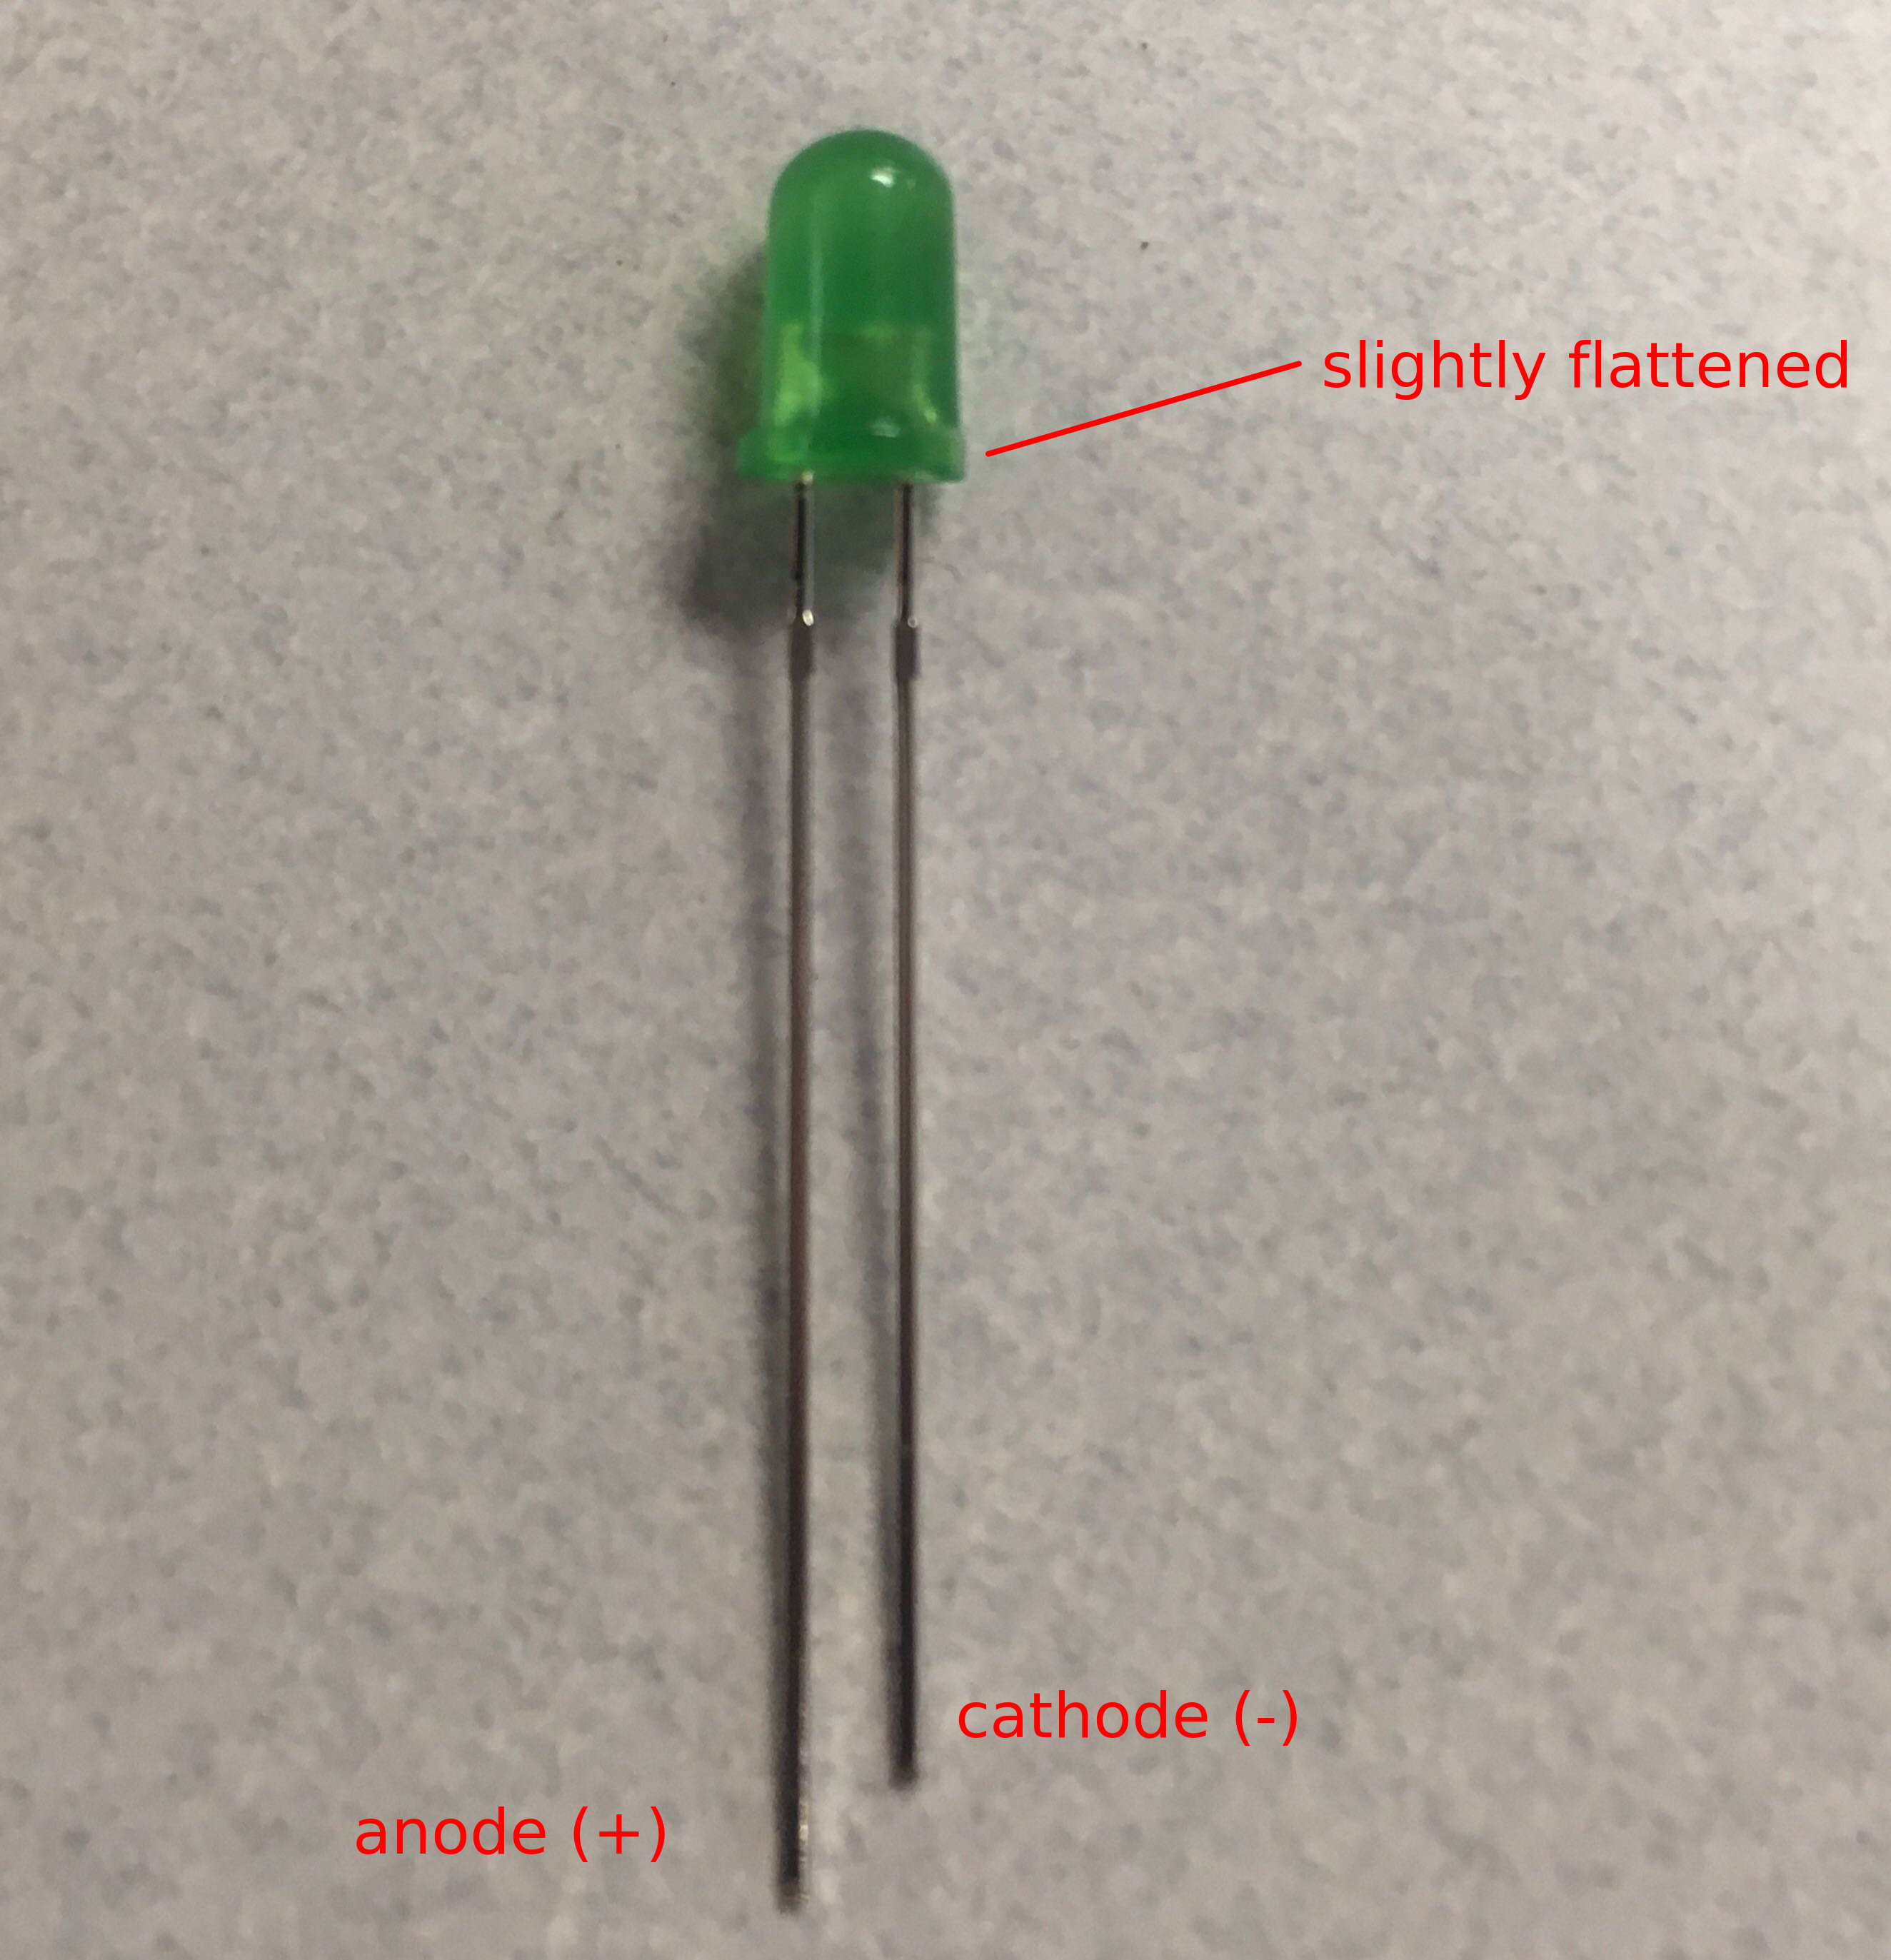
\includegraphics[max width = 0.5\textwidth]{led.jpg}

	\caption{Photo showing the anode and cathode of an LED.}

\end{figure}

\begin{figure}[H]
	\centering

	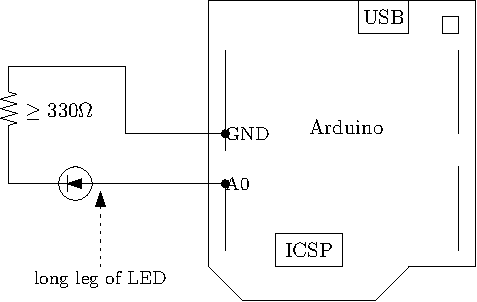
\includegraphics[max width = 0.7\textwidth]{wiring_diagram.pdf}

	\caption{Wiring diagram for LED blink program.}

\end{figure}

You should also connect the USB cable from your Arduino to your workstation.
This is how you will connect to the UART console.

Finally, connect the AVRIce programmer to your workstation, and the programming
cable to the Arduino. Remember that the tab on the programming cable should be
facing the interior of the Arduino board.

\begin{figure}[H]
	\centering

	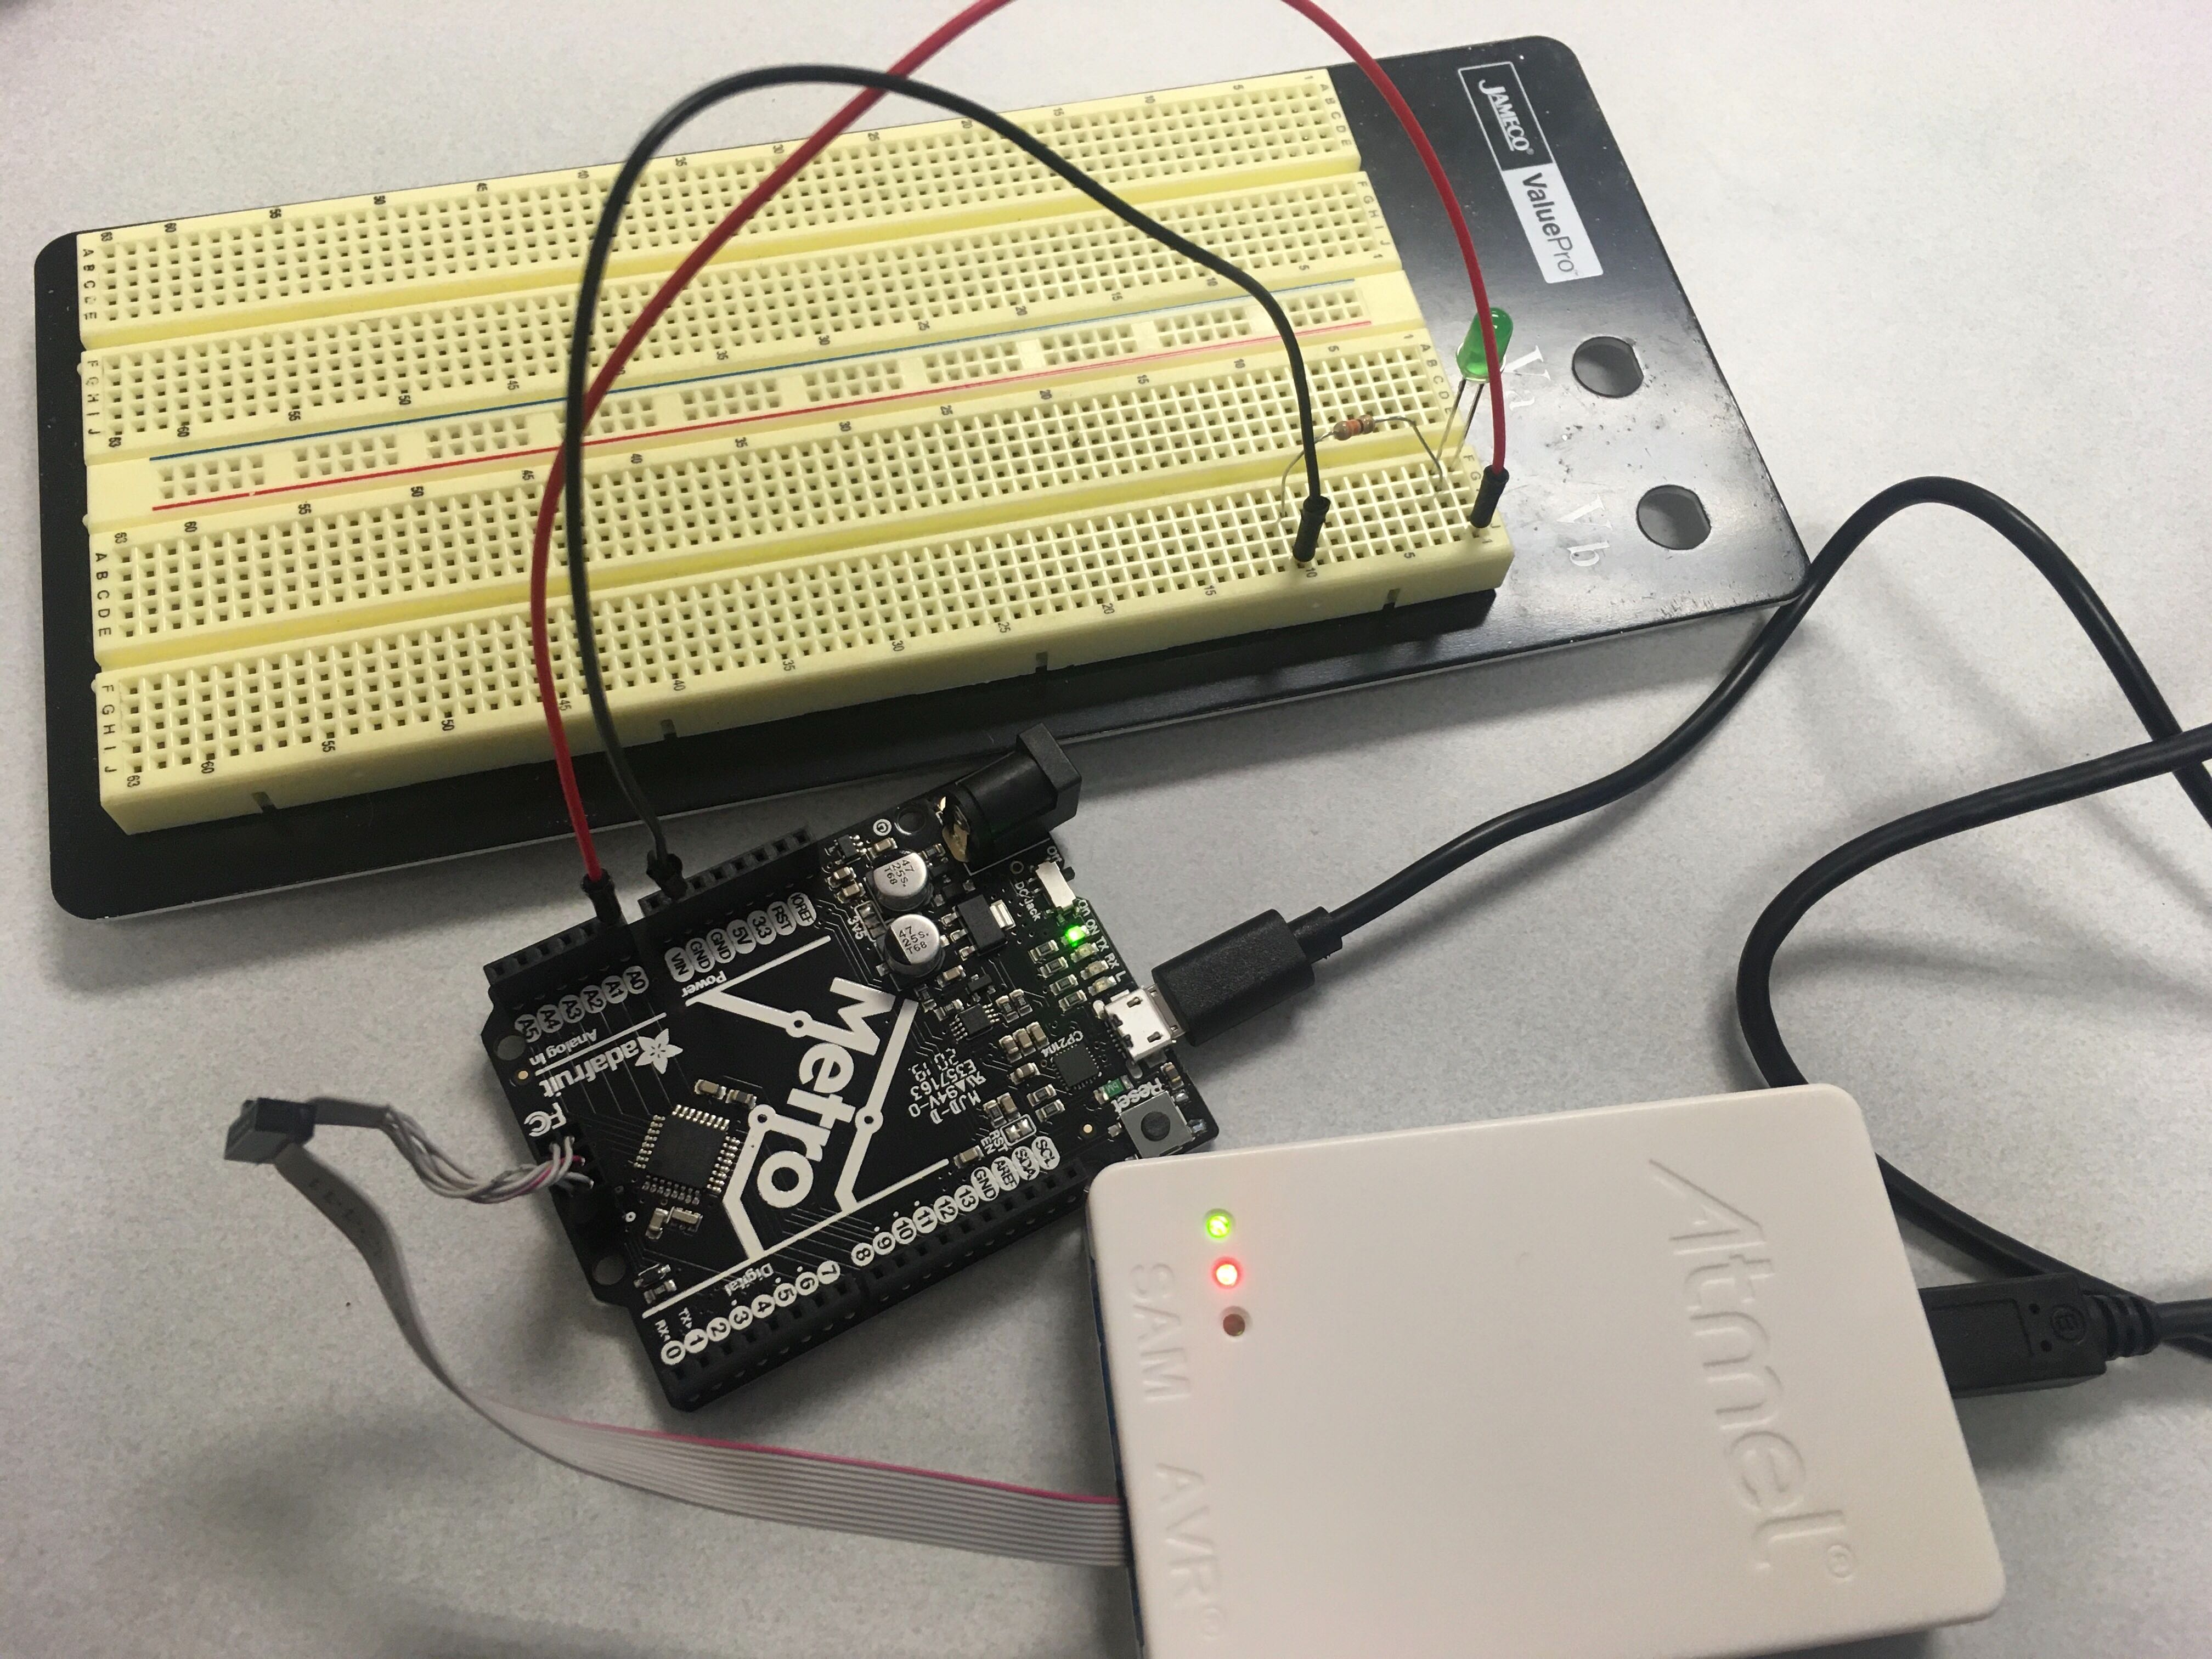
\includegraphics[max width = 0.7\textwidth]{wiring.jpg}

	\caption{Photograph showing correctly wired project.}

\end{figure}

If you want to validate your wiring, you can use \texttt{make reference} which
will flash the reference solution to the board. It should start in a
non-blinking state, and will allow blinking to be toggled via the UART console
as described in part C.

\subsection{Requirements}

\begin{itemize}

	\item (A.1) LED blinks continuously, remaining lit for roughly
	$\frac{1}{2}$ second, and remaining off for roughly the same amount
	of time.

\end{itemize}

\subsection{Grading}

You do not need to submit any code for this portion. During lab, office hours,
or by appointment, demonstrate your project to your TA or instructor.

\section{Part B: UART "hello world"}

\subsection{Requirements}

\begin{itemize}

	\item (B.1) When the AVR is reset, the message "Hello World!" is
	displayed via an attached UART console. The UART configuration
	57600 8N1 should be used.

\end{itemize}

\subsection{Grading}

You do not need to submit any code for this portion. During lab, office hours,
or by appointment, demonstrate your project to your TA or instructor.

\section{Part C: UART Control Console}

\subsection{Requirements}

\begin{itemize}

	\item (C.1) When the AVR is ready to accept input, a prompt of your
	choice (for example: \texttt{ready> }) should be displayed indicting the
	user may enter a command.

	\item (C.2) When the user enters the command \texttt{on}, the LED
	should begin blinking as in Part A, and should continue to do so
	until another command is entered or the AVR is reset.

	\item (C.3) When the user enters the command \texttt{off}, the LED
	should stop blinking, and remain unlit indefinitely until another
	command is entered or the AVR is reset.

	\item (C.4) If any other text string is entered, an informative error
	message should be displayed via the console. The state of the LED
	should remain unchanged (i.e. if the LED was blinking, it should
	continue to do so). You may assume no command will be entered which is
	more than 64 characters in length.

	\item (C.5) When the AVR is reset, the LED should be in the "off"
	state.

\end{itemize}

\subsection{Grading}

During lab, office hours, or by appointment, demonstrate your project to your
TA or instructor.  You will also submit your code for this portion of the
assignment via Moodle.  \textbf{Please pack your code using the command
\texttt{make pack}.  Incorrectly packed project submissions will not be
graded.}

Note that the \texttt{make pack} script will not allow you to pack your code if
the \texttt{reflection.txt} file is unmodified - if you want to submit part C
without starting your reflection, then just modify it with a line that says "I
will complete my reflection in Part D" (or something to that effect so that we
know you have acknowledge you need to complete it).

\subsection{Background}

Part C differs from the first two parts of the lab, in that two separate
concerns are present - blinking the LED and interacting with the UART. There
are several ways that one might choose to address this, and no specific method
is prescribed for the purposes of this lab. It is probably easiest to use the
static scheduling approach, but the interrupt-driven approach will be used in
future labs, so you may wish to get a head start by using that.

The first main general style of approaching this problem is \textbf{static
scheduling}. You might simple have a single loop that runs forever. In each
loop iteration, check if the LED needs to turn on, turn off, or stay the same
and do so if necessary, then check if there is a character ready to read from
UART and append it to a read buffer, then check if the read buffer has enough
data to process and so on. This approach has several benefits: it is simple to
understand and implement, it is easy to predict how long each loop iteration
will take, and operation will always be fully deterministic.

A more advanced approach would be \textbf{interrupt driven}. This could be done
by either utilizing the ISR\footnote{Interrupt Service Routine} which runs when
UART data is ready and using this ISR for command processing, or by using one
of the timer/counter interrupts to control the LED while polling the UART
controller synchronously.

There are of course other ways of solving this problem. On a more powerful
processor, one might use time-division multiplexing to implement several
threads of execution, each implementing synchronous polling. On devices with
multiple processing cores, one could simply have two separate threads running
in parallel with no special logic required.

\section{Part D: Software UART}

\subsection{Requirements}

\begin{itemize}

	\item (D.1) from the perspective of the user, your project should work
		exactly the same as in part C.

	\item (D.2) the transmit functionality of your project (i.e.
		\texttt{uart\_putchar()}) must be implemented using software,
		\textbf{not} the hardware UART controller.

	\item (D.3) said software transmit functionality should operate at a
		reasonable baud rate (at least 9.6k baud). The reference
		implementation runs at 57.6k baud.

	\item (D.4) your project should continue to use the hardware UART
		controller for receiving data from the console.

\end{itemize}

\subsection{Grading}

During lab, office hours, or by appointment, demonstrate your project to your
TA or instructor.  You will also submit your code for this portion of the
assignment via Moodle.  \textbf{Please pack your code using the command
\texttt{make pack}.  Incorrectly packed project submissions will not be
graded.}

\subsection{Background}

In this part of the assignment, you are asked to implement a "bit-banged"
implementation of UART transmission. "bit-banging" is the practice of
implementing a communications protocol by directly manipulating GPIO pins,
rather than using a hardware controller. This can be a powerful and useful
technique. We will use this method later in the course to interface with our
WiFi adapter while still maintaining a separate debug output by using both the
hardware controller and our bit-banged implementation simultaneously.

Note that you should use PD1 (Arduino digital Pin 1) as the TX pin for your
software UART implementation (as you need only implement TX functionality, you
need not allocate a TX pin). This is because it will allow you to take
advantage of the UART to USB converter built into the Arduino.

You will want accurate delay functions in order to implement this
functionality. You should consider using
\texttt{util/delay.h}\footnote{\url{https://www.nongnu.org/avr-libc/user-manual/group__util__delay.html}}.
This provides functions for delaying by a number of milliseconds or
microseconds.

\section{Reflection}

\textbf{You should submit your answers by editing \texttt{reflection.txt} to
include them before you run \texttt{make pack}}.  There is no specific
requirement for word or page count, but roughly 1-3 paragraphs are expected in
response to each question. Note that your reflection will be graded with your
submission to part D.

\subsection{Question 1}

A fellow \course \hspace{1pt} student says they are pretty sure they have
implemented Part B correctly, but their terminal just shows random junk.
Speculate on the cause of this problem.

\subsection{Question 2}

How did you choose to solve the problem in Part C of managing two separate
tasks at the same time? Why did you select this approach?

\subsection{Question 3}

Suppose you were tasked with implementing a new feature in your project where a
user could also enter a command \texttt{set X} with \texttt{X} being a number
of milliseconds specifying the total period of the LED blink cycle. In other
words, when the LED is blinking, it should stay on for $\frac{\texttt{X}}{2}$ ms,
rather than a half second. Briefly describe how you would implement this
feature.

\section{Rubric}

\begin{itemize}

	\item 10 pts - Part A demonstration

	\item 10 pts - Part B demonstration

	\item 10 pts - Part C demonstration

	\item 15 pts - Part C code review

	\begin{itemize}

		\item 5 pts - Should interface with the UART controller (no
		third party libraries, no bit-banging).

		\item 5 pts - Set up \texttt{stdin} and \texttt{stdout} so that
		\texttt{printf()} works.

		\item 5 pts - Style.

	\end{itemize}

	\item 10 pts - Part D demonstration

	\item 15 pts - Part D code review

	\begin{itemize}

		\item 5 pts - Should implement UART transmit using bit-banging,
			and UART receive using the hardware controller.

		\item 5 pts - All other aspects from part C should still work.

		\item 5 pts - Style.

	\end{itemize}


	\item 30 pts - Reflection (10 pts per question)

\end{itemize}

\textbf{Maximum number of points possible: 100.}

Keep in mind that some items not listed on the rubric may cause you to loose
points, including cheating, submitting code which is inconsistent with what you
have demonstrating, plagiarizing code or reflection content, etc.


\end{document}
